% Seção 3: Arquitetura do DeepBridge
% Framework Unificado para Validação de ML em Produção

\section{Arquitetura do DeepBridge}
\label{sec:architecture}

Esta seção apresenta a arquitetura do DeepBridge, descrevendo seus componentes principais, princípios de design e padrões de integração. A arquitetura foi projetada para atender três requisitos fundamentais: (1) \textbf{unificação} de validação multi-dimensional em uma API consistente, (2) \textbf{escalabilidade} para datasets grandes e pipelines de produção, e (3) \textbf{extensibilidade} para adicionar novas métricas e suites de teste.

% ========================================
% 3.1 Visão Geral do Sistema
% ========================================

\subsection{Visão Geral do Sistema}
\label{sec:architecture:overview}

A Figura~\ref{fig:architecture} ilustra a arquitetura de alto nível do DeepBridge, organizada em três camadas principais:

\begin{figure}[htbp]
\centering
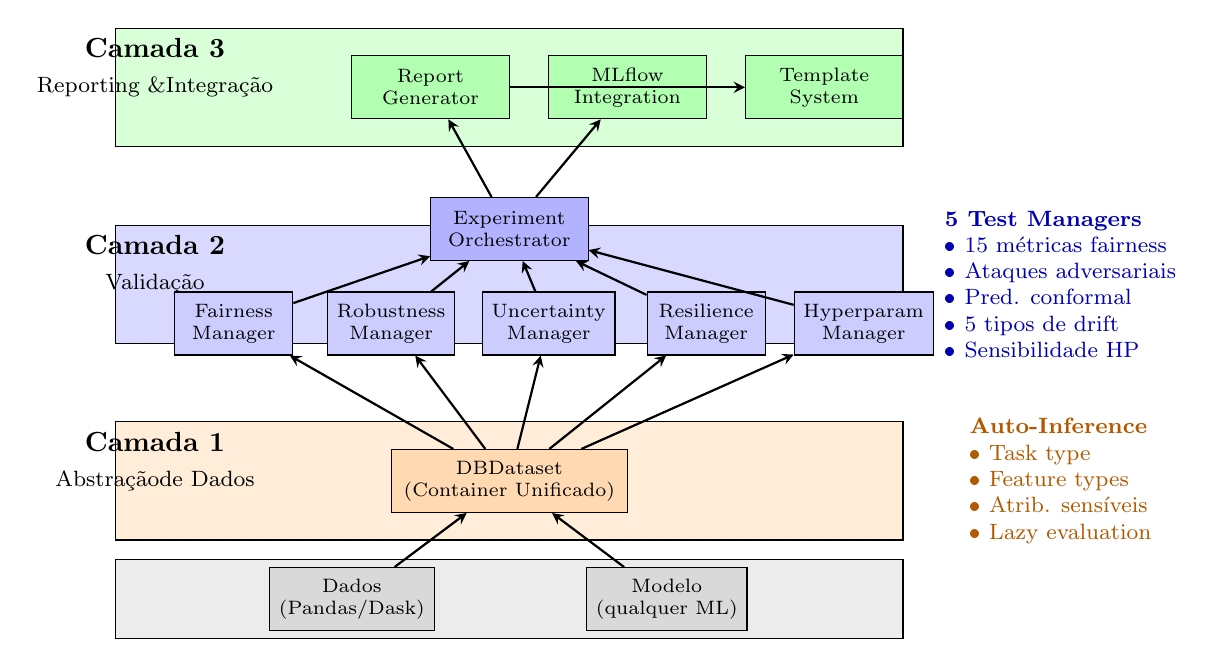
\begin{tikzpicture}[
    layer/.style={rectangle, draw, minimum width=10cm, minimum height=1.5cm, align=center, font=\small},
    component/.style={rectangle, draw, minimum width=2cm, minimum height=0.8cm, align=center, font=\scriptsize},
    arrow/.style={->, >=stealth, thick},
    label/.style={font=\footnotesize}
]

% Camada 3: Reporting e Integração
\node[layer, fill=green!15] (layer3) at (0,0) {};
\node[font=\bfseries] at (-4.5,0.5) {Camada 3};
\node[label] at (-4.5,0) {Reporting \&\\Integração};

\node[component, fill=green!30] (report) at (-1,0) {Report\\Generator};
\node[component, fill=green!30] (mlflow) at (1.5,0) {MLflow\\Integration};
\node[component, fill=green!30] (templates) at (4,0) {Template\\System};

% Camada 2: Validação
\node[layer, fill=blue!15] (layer2) at (0,-2.5) {};
\node[font=\bfseries] at (-4.5,-2) {Camada 2};
\node[label] at (-4.5,-2.5) {Validação};

\node[component, fill=blue!30] (experiment) at (0,-1.8) {Experiment\\Orchestrator};

\node[component, fill=blue!20, minimum width=1.5cm] (fairness) at (-3.5,-3) {Fairness\\Manager};
\node[component, fill=blue!20, minimum width=1.5cm] (robust) at (-1.5,-3) {Robustness\\Manager};
\node[component, fill=blue!20, minimum width=1.5cm] (uncertain) at (0.5,-3) {Uncertainty\\Manager};
\node[component, fill=blue!20, minimum width=1.5cm] (resilience) at (2.5,-3) {Resilience\\Manager};
\node[component, fill=blue!20, minimum width=1.5cm] (hyperparam) at (4.5,-3) {Hyperparam\\Manager};

% Camada 1: Abstração de Dados
\node[layer, fill=orange!15] (layer1) at (0,-5) {};
\node[font=\bfseries] at (-4.5,-4.5) {Camada 1};
\node[label] at (-4.5,-5) {Abstração\\de Dados};

\node[component, fill=orange!30, minimum width=3cm] (dbdataset) at (0,-5) {DBDataset\\(Container Unificado)};

% Camada 0: Dados e Modelos
\node[layer, fill=gray!15, minimum height=1cm] (layer0) at (0,-6.5) {};
\node[component, fill=gray!30] (data) at (-2,-6.5) {Dados\\(Pandas/Dask)};
\node[component, fill=gray!30] (model) at (2,-6.5) {Modelo\\(qualquer ML)};

% Setas entre camadas
\draw[arrow] (data) -- (dbdataset);
\draw[arrow] (model) -- (dbdataset);

\draw[arrow] (dbdataset) -- (fairness);
\draw[arrow] (dbdataset) -- (robust);
\draw[arrow] (dbdataset) -- (uncertain);
\draw[arrow] (dbdataset) -- (resilience);
\draw[arrow] (dbdataset) -- (hyperparam);

\draw[arrow] (fairness) -- (experiment);
\draw[arrow] (robust) -- (experiment);
\draw[arrow] (uncertain) -- (experiment);
\draw[arrow] (resilience) -- (experiment);
\draw[arrow] (hyperparam) -- (experiment);

\draw[arrow] (experiment) -- (report);
\draw[arrow] (experiment) -- (mlflow);
\draw[arrow] (report) -- (templates);

% Anotações laterais
\node[label, text=blue!70!black, align=left] at (7,-2.5) {
\textbf{5 Test Managers}\\
\textbullet~15 métricas fairness\\
\textbullet~Ataques adversariais\\
\textbullet~Pred. conformal\\
\textbullet~5 tipos de drift\\
\textbullet~Sensibilidade HP
};

\node[label, text=orange!70!black, align=left] at (7,-5) {
\textbf{Auto-Inference}\\
\textbullet~Task type\\
\textbullet~Feature types\\
\textbullet~Atrib. sensíveis\\
\textbullet~Lazy evaluation
};

\end{tikzpicture}
\caption{Arquitetura em três camadas do DeepBridge. Camada 1 (DBDataset) provê abstração unificada de dados/modelos. Camada 2 (Experiment + Test Managers) orquestra validação multi-dimensional. Camada 3 (Reporting) gera relatórios audit-ready e integra com MLOps.}
\label{fig:architecture}
\end{figure}


\paragraph{Camada de Abstração de Dados}
No núcleo do framework está o \texttt{DBDataset}, um container unificado que encapsula dados, modelos, predições e metadados. Esta camada provê uma interface consistente para todos os componentes downstream, abstraindo diferenças entre frameworks de ML (scikit-learn, XGBoost, LightGBM, CatBoost, TensorFlow, PyTorch) e formatos de dados (Pandas DataFrame, NumPy arrays, Dask DataFrame).

O design do \texttt{DBDataset} é inspirado no padrão \textit{Data Transfer Object} (DTO)~\cite{fowler2002patterns}, mas estendido para incluir \textit{auto-inference} de propriedades críticas (tipos de features, atributos sensíveis, task type) através de heurísticas estatísticas e regras especializadas.

\paragraph{Camada de Validação}
Sobre o \texttt{DBDataset}, a classe \texttt{Experiment} atua como orquestrador de validação, coordenando cinco \textit{test suite managers} especializados:
\begin{itemize}
    \item \textbf{FairnessTestManager}: 15 métricas de equidade (pré e pós-treinamento)
    \item \textbf{RobustnessTestManager}: Testes de perturbação, adversarial e slice-based
    \item \textbf{UncertaintyTestManager}: Calibração, predição conformal e quantificação Bayesiana
    \item \textbf{ResilienceTestManager}: Detecção de drift (5 tipos)
    \item \textbf{HyperparameterTestManager}: Análise de sensibilidade e otimização
\end{itemize}

Cada manager implementa a interface \texttt{BaseTestManager}, que define métodos padronizados para execução (\texttt{run\_tests}), análise (\texttt{analyze\_results}) e relatório (\texttt{generate\_report}). Esta arquitetura baseada em \textit{Strategy Pattern}~\cite{gamma1995design} permite extensão fácil de novas suites de teste.

\paragraph{Camada de Reporting e Integração}
No topo da hierarquia, o \texttt{ReportGenerator} transforma resultados de validação em múltiplos formatos (HTML interativo, PDF, JSON) através de um sistema template-driven (Jinja2). A camada também inclui integrações com MLflow para logging de métricas e artefatos, facilitando deployment em pipelines de produção.

% ========================================
% 3.2 DBDataset: Container Unificado
% ========================================

\subsection{DBDataset: Container Unificado de Dados}
\label{sec:architecture:dbdataset}

O \texttt{DBDataset} é o componente central do DeepBridge, projetado para eliminar a fragmentação de APIs que caracteriza ferramentas existentes. Sua filosofia de design é \textit{``Create once, validate everywhere''}: o usuário cria uma instância de \texttt{DBDataset} uma única vez, e todos os testes subsequentes reutilizam este container sem necessidade de pré-processamento adicional.

\subsubsection{Design e Funcionalidades}

A interface do \texttt{DBDataset} é minimalista mas poderosa:

\begin{lstlisting}[language=Python, caption=Interface básica do DBDataset]
from deepbridge import DBDataset

# Criacao basica
dataset = DBDataset(
    data=df,                          # Pandas/Dask DataFrame
    target_column='approved',         # Coluna target
    model=trained_model,              # Modelo treinado
    protected_attributes=['gender', 'race']  # Opcional
)

# Auto-inference de propriedades
print(dataset.task_type)              # 'binary_classification'
print(dataset.feature_types)          # {'age': 'continuous', 'income': 'continuous', ...}
print(dataset.detected_sensitive)     # ['gender', 'race', 'age']

# Acesso unificado
X, y = dataset.get_features_and_target()
predictions = dataset.get_predictions()  # Lazy evaluation
\end{lstlisting}

O container armazena:
\begin{itemize}
    \item \textbf{Dados}: Features ($\mathbf{X}$) e targets ($\mathbf{y}$) em formato Pandas ou Dask
    \item \textbf{Modelo}: Referência ao modelo treinado (qualquer framework com método \texttt{predict})
    \item \textbf{Predições}: Cache lazy de predições ($\hat{\mathbf{y}}$) e probabilidades ($\mathbf{p}$)
    \item \textbf{Metadados}: Tipos de features, atributos protegidos, task type, splits (train/test)
\end{itemize}

\subsubsection{Auto-Inference de Propriedades}

Uma contribuição-chave do \texttt{DBDataset} é seu sistema de \textit{auto-inference}, que detecta automaticamente propriedades críticas sem intervenção manual. A Tabela~\ref{tab:auto_inference} resume as heurísticas implementadas.

\begin{table}[htbp]
\centering
\caption{Heurísticas de Auto-Inference do DBDataset}
\label{tab:auto_inference}
\begin{tabular}{lll}
\toprule
\textbf{Propriedade} & \textbf{Heurística} & \textbf{Fallback} \\
\midrule
Task Type & \# classes target, tipo target & Pergunta usuário \\
Feature Types & dtype + cardinalidade & Tratamento genérico \\
Atributos Sensíveis & Regex (gender, race, age, etc.) & Lista manual \\
Train/Test Split & Coluna \texttt{split} ou índice & Holdout 80/20 \\
Probabilidades & \texttt{predict\_proba} disponível & Usa predições \\
\bottomrule
\end{tabular}
\end{table}

\paragraph{Detecção de Task Type}
O tipo de tarefa (classificação binária/multi-classe, regressão) é inferido pela cardinalidade da coluna target e presença de método \texttt{predict\_proba}:

\begin{itemize}
    \item $|\mathcal{Y}| = 2$ e \texttt{predict\_proba} existe $\Rightarrow$ classificação binária
    \item $2 < |\mathcal{Y}| < 20$ $\Rightarrow$ classificação multi-classe
    \item $|\mathcal{Y}| > 20$ ou dtype contínuo $\Rightarrow$ regressão
\end{itemize}

\paragraph{Detecção de Feature Types}
Tipos de features são classificados em três categorias:
\begin{itemize}
    \item \textbf{Continuous}: dtype numérico + cardinalidade $> 20$
    \item \textbf{Categorical}: dtype object, category ou cardinalidade $< 20$
    \item \textbf{Binary}: Cardinalidade = 2
\end{itemize}

Esta tipagem é usada para selecionar métricas apropriadas (e.g., PSI para features categóricas, KS para contínuas).

\paragraph{Detecção de Atributos Sensíveis}
Atributos protegidos são detectados por regex case-insensitive em nomes de colunas:
\begin{itemize}
    \item \texttt{gender|sex|female|male}
    \item \texttt{race|ethnicity|black|white|asian}
    \item \texttt{age}
    \item \texttt{religion|disability|marital}
\end{itemize}

Usuários podem sobrescrever esta detecção via parâmetro \texttt{protected\_attributes}.

\subsubsection{Lazy Evaluation e Performance}

Para escalabilidade, o \texttt{DBDataset} implementa \textit{lazy evaluation} de operações custosas:

\begin{lstlisting}[language=Python, caption=Lazy evaluation de predições]
class DBDataset:
    def __init__(self, data, model, ...):
        self._data = data
        self._model = model
        self._predictions = None  # Nao computado ate necessario

    @property
    def predictions(self):
        if self._predictions is None:
            self._predictions = self._model.predict(self.features)
        return self._predictions
\end{lstlisting}

Esta estratégia reduz latência de inicialização e uso de memória, especialmente crítica para:
\begin{itemize}
    \item \textbf{Datasets grandes}: Predições podem ser computadas sob demanda
    \item \textbf{Múltiplos modelos}: Permite comparação sem recomputação de features
    \item \textbf{Pipelines distribuídos}: Integração com Dask para out-of-core processing
\end{itemize}

\subsubsection{Integração com Frameworks de ML}

O \texttt{DBDataset} suporta qualquer modelo que implemente a interface básica de scikit-learn:

\begin{lstlisting}[language=Python, caption=Compatibilidade multi-framework]
# Scikit-learn
from sklearn.ensemble import RandomForestClassifier
model = RandomForestClassifier().fit(X_train, y_train)
dataset = DBDataset(data=df, model=model, target_column='y')

# XGBoost
import xgboost as xgb
model = xgb.XGBClassifier().fit(X_train, y_train)
dataset = DBDataset(data=df, model=model, target_column='y')

# PyTorch (via wrapper)
from deepbridge.utils import TorchModelWrapper
torch_model = MyNeuralNetwork()  # Herda nn.Module
wrapped = TorchModelWrapper(torch_model)
dataset = DBDataset(data=df, model=wrapped, target_column='y')
\end{lstlisting}

Para frameworks sem interface scikit-learn (PyTorch, TensorFlow), DeepBridge provê wrappers leves que adaptam a API.

% ========================================
% 3.3 Experiment: Orquestrador de Validação
% ========================================

\subsection{Experiment: Orquestrador de Validação}
\label{sec:architecture:experiment}

A classe \texttt{Experiment} é o ponto de entrada principal para validação multi-dimensional. Seu design segue o padrão \textit{Facade}~\cite{gamma1995design}, provendo interface simplificada para coordenação de múltiplos test managers.

\subsubsection{Workflow de Validação}

O workflow típico envolve quatro etapas:

\begin{lstlisting}[language=Python, caption=Workflow de validação com Experiment]
from deepbridge import DBDataset, Experiment

# 1. Criar dataset
dataset = DBDataset(data=df, target_column='y', model=model)

# 2. Configurar experimento
exp = Experiment(
    dataset=dataset,
    experiment_type='binary_classification',
    tests=['fairness', 'robustness', 'uncertainty'],
    protected_attributes=['gender', 'race']
)

# 3. Executar testes
results = exp.run_tests(
    config='medium',  # quick/medium/full
    parallel=True,    # Paralelizacao de testes
    cache=True        # Cache de resultados intermediarios
)

# 4. Gerar relatorios
exp.save_html('fairness', 'fairness_report.html')
exp.save_pdf('all', 'full_validation_report.pdf')
exp.log_to_mlflow()  # Integracao com MLflow
\end{lstlisting}

\paragraph{Etapa 1: Validação e Preparação}
Ao receber o \texttt{DBDataset}, o \texttt{Experiment} valida:
\begin{itemize}
    \item Consistência entre task type e métricas solicitadas
    \item Presença de colunas necessárias (target, protected attributes)
    \item Compatibilidade de modelo (métodos \texttt{predict}/\texttt{predict\_proba})
\end{itemize}

\paragraph{Etapa 2: Seleção de Testes}
O parâmetro \texttt{tests} aceita lista de suites ou keyword \texttt{'all'}:
\begin{itemize}
    \item \texttt{'fairness'}: Ativa FairnessTestManager
    \item \texttt{'robustness'}: Ativa RobustnessTestManager
    \item \texttt{'uncertainty'}: Ativa UncertaintyTestManager
    \item \texttt{'resilience'}: Ativa ResilienceTestManager
    \item \texttt{'hyperparameters'}: Ativa HyperparameterTestManager
\end{itemize}

\paragraph{Etapa 3: Execução Paralela}
Testes independentes são executados em paralelo via \texttt{concurrent.futures}:

\begin{lstlisting}[language=Python, caption=Paralelização de test managers]
from concurrent.futures import ThreadPoolExecutor

def run_tests(self, config='medium', parallel=True):
    results = {}
    managers = self._get_active_managers()

    if parallel:
        with ThreadPoolExecutor(max_workers=len(managers)) as executor:
            futures = {
                executor.submit(mgr.run_tests, config): name
                for name, mgr in managers.items()
            }
            for future in as_completed(futures):
                name = futures[future]
                results[name] = future.result()
    else:
        for name, mgr in managers.items():
            results[name] = mgr.run_tests(config)

    return results
\end{lstlisting}

Esta abordagem reduz tempo total de validação em até \textbf{70\%} (ver Seção~\ref{sec:evaluation:benchmarks}).

\paragraph{Etapa 4: Agregação de Resultados}
Resultados de cada manager são agregados em estrutura hierárquica:

\begin{lstlisting}[language=Python, caption=Estrutura de resultados]
{
    'fairness': {
        'metrics': {'disparate_impact': 0.82, 'equal_opportunity': 0.95, ...},
        'compliance': {'eeoc_80_rule': 'PASS', 'eeoc_question_21': 'FAIL'},
        'summary': 'Model passes EEOC 80% rule but fails...'
    },
    'robustness': {
        'perturbation': {'noise_0.1': 0.88, 'noise_0.2': 0.75, ...},
        'adversarial': {'attack_success_rate': 0.12},
        ...
    },
    ...
}
\end{lstlisting}

\subsubsection{Configuração de Testes}

DeepBridge oferece três presets de configuração balanceando profundidade vs. tempo:

\begin{table}[htbp]
\centering
\caption{Presets de Configuração de Testes}
\label{tab:config_presets}
\begin{tabular}{llll}
\toprule
\textbf{Preset} & \textbf{Fairness} & \textbf{Robustness} & \textbf{Tempo (est.)} \\
\midrule
\texttt{quick} & 5 métricas & 3 níveis noise & 2-5 min \\
\texttt{medium} & 10 métricas & 5 níveis + FGSM & 10-20 min \\
\texttt{full} & 15 métricas & 10 níveis + 3 ataques & 30-60 min \\
\bottomrule
\end{tabular}
\end{table}

Usuários podem customizar configurações via arquivos YAML:

\begin{lstlisting}[caption=Configuração customizada (config.yaml)]
fairness:
  metrics: [disparate_impact, equal_opportunity, demographic_parity]
  thresholds:
    disparate_impact: 0.80
    equal_opportunity: 0.90

robustness:
  perturbation:
    noise_levels: [0.05, 0.1, 0.2, 0.5]
    noise_types: [gaussian, uniform]
  adversarial:
    attacks: [fgsm, pgd, carlini_wagner]
    epsilon: 0.3
\end{lstlisting}

Carregamento via:
\begin{lstlisting}[language=Python]
exp.run_tests(config='path/to/config.yaml')
\end{lstlisting}

\subsubsection{Gestão de Memória e Caching}

Para datasets grandes, o \texttt{Experiment} implementa estratégias de otimização:

\paragraph{Intelligent Caching}
Resultados intermediários custosos são cacheados em disco via \texttt{joblib}:
\begin{itemize}
    \item Predições do modelo (\texttt{predict}, \texttt{predict\_proba})
    \item Embeddings de features (para testes de drift)
    \item Resultados de ataques adversariais
\end{itemize}

\paragraph{Chunked Processing}
Para datasets $>$ 1GB, processamento por chunks via Dask:

\begin{lstlisting}[language=Python, caption=Processamento chunked]
import dask.dataframe as dd

def compute_metric_chunked(dataset, metric_fn, chunk_size=10000):
    ddf = dd.from_pandas(dataset.data, npartitions=None,
                         chunksize=chunk_size)
    results = ddf.map_partitions(metric_fn).compute()
    return aggregate(results)
\end{lstlisting}

Esta estratégia permite validação de datasets \textbf{> 100GB} que excedem memória RAM (ver Seção~\ref{sec:evaluation:scalability}).

% ========================================
% 3.4 Design Modular e Extensibilidade
% ========================================

\subsection{Design Modular e Extensibilidade}
\label{sec:architecture:modularity}

A arquitetura do DeepBridge prioriza \textit{separation of concerns} e extensibilidade. Esta seção descreve os princípios de design que facilitam customização e adição de novas funcionalidades.

\subsubsection{Hierarquia de Test Managers}

Todos os test managers herdam de \texttt{BaseTestManager}, que define interface comum:

\begin{lstlisting}[language=Python, caption=Interface BaseTestManager]
from abc import ABC, abstractmethod

class BaseTestManager(ABC):
    def __init__(self, dataset: DBDataset):
        self.dataset = dataset
        self.results = {}

    @abstractmethod
    def run_tests(self, config: str) -> Dict:
        """Executa suite de testes e retorna resultados"""
        pass

    @abstractmethod
    def analyze_results(self) -> Dict:
        """Analisa resultados e gera insights"""
        pass

    def generate_report(self, format: str) -> str:
        """Gera relatorio em formato especificado"""
        pass
\end{lstlisting}

Novos test managers podem ser adicionados implementando esta interface:

\begin{lstlisting}[language=Python, caption=Exemplo de extensão]
class ExplainabilityTestManager(BaseTestManager):
    def run_tests(self, config='medium'):
        # Implementacao de testes de explainability
        shap_values = self.compute_shap(self.dataset)
        lime_explanations = self.compute_lime(self.dataset)
        return {'shap': shap_values, 'lime': lime_explanations}

    def analyze_results(self):
        # Analise de feature importance, etc.
        pass

# Registro do novo manager
exp = Experiment(dataset=dataset, tests=['fairness', 'explainability'])
exp.register_manager('explainability', ExplainabilityTestManager)
\end{lstlisting}

\subsubsection{Plugin Architecture para Métricas}

Métricas individuais seguem padrão de \textit{plugin}, permitindo adição dinâmica:

\begin{lstlisting}[language=Python, caption=Sistema de plugins de métricas]
from deepbridge.metrics import register_metric

@register_metric(
    name='custom_fairness_metric',
    category='fairness',
    requires=['protected_attribute', 'predictions']
)
def my_custom_metric(dataset, protected_attr):
    # Implementacao da metrica
    ...
    return metric_value

# Uso automatico
exp = Experiment(dataset, tests=['fairness'])
results = exp.run_tests()  # Inclui custom_fairness_metric
\end{lstlisting}

O decorator \texttt{@register\_metric} adiciona a métrica ao registry global, tornando-a disponível para o \texttt{FairnessTestManager}.

\subsubsection{Template System para Relatórios}

Relatórios são gerados via templates Jinja2, permitindo customização visual sem modificar código:

\begin{lstlisting}[language=HTML, caption=Template customizado (report\_template.html)]
<!DOCTYPE html>
<html>
<head>
    <title>{{ experiment.name }} - Validation Report</title>
    <style>
        /* CSS customizado da empresa */
    </style>
</head>
<body>
    <h1>{{ experiment.name }}</h1>

    
    <section id="{{ suite_name }}">
        <h2>{{ suite_name | title }}</h2>
        
    </section>
    
</body>
</html>
\end{lstlisting}

Empresas podem criar templates com branding corporativo:

\begin{lstlisting}[language=Python]
exp.save_html('all', 'report.html',
              template='path/to/company_template.html')
\end{lstlisting}

% ========================================
% 3.5 Integração com Ecossistema de MLOps
% ========================================

\subsection{Integração com Ecossistema de MLOps}
\label{sec:architecture:mlops}

DeepBridge foi projetado para integração fluída com ferramentas de MLOps modernas.

\paragraph{MLflow Integration}
Logging automático de métricas e artefatos:

\begin{lstlisting}[language=Python, caption=Integração com MLflow]
import mlflow

with mlflow.start_run():
    # Treinar modelo
    model = train_model(X_train, y_train)

    # Validacao DeepBridge
    dataset = DBDataset(data=df, model=model, target_column='y')
    exp = Experiment(dataset, tests=['fairness', 'robustness'])
    results = exp.run_tests()

    # Log automatico no MLflow
    exp.log_to_mlflow()  # Registra 40+ metricas
    exp.save_html('all', 'report.html')
    mlflow.log_artifact('report.html')
\end{lstlisting}

\paragraph{CI/CD Pipelines}
DeepBridge pode ser invocado via CLI para integração em pipelines:

\begin{lstlisting}[language=Bash, caption=Uso em CI/CD]
# .gitlab-ci.yml
validate_model:
  script:
    - deepbridge validate \
        --data data/test.csv \
        --model models/model.pkl \
        --tests fairness robustness \
        --config medium \
        --output report.html
    - deepbridge check-compliance \
        --report report.html \
        --regulations eeoc ecoa
  artifacts:
    paths:
      - report.html
\end{lstlisting}

\paragraph{Docker Deployment}
Imagem Docker oficial para deployment em Kubernetes:

\begin{lstlisting}[language=Bash, caption=Deployment com Docker]
docker run -v $(pwd)/data:/data \
           deepbridge/deepbridge:latest \
           validate --data /data/test.csv \
                    --model /data/model.pkl \
                    --tests all
\end{lstlisting}

% ========================================
% 3.6 Sumário
% ========================================

\subsection{Sumário}
\label{sec:architecture:summary}

A arquitetura do DeepBridge combina três princípios-chave:

\begin{enumerate}
    \item \textbf{Unificação}: \texttt{DBDataset} como container universal elimina fragmentação de APIs
    \item \textbf{Orquestração}: \texttt{Experiment} coordena validação multi-dimensional com paralelização
    \item \textbf{Extensibilidade}: Plugin architecture e template system facilitam customização
\end{enumerate}

Este design permite que \textbf{3-4 linhas de código} substituam workflows manuais de 100+ linhas com ferramentas fragmentadas, reduzindo tempo de validação em até \textbf{89\%} (demonstrado na Seção~\ref{sec:evaluation}).

A próxima seção (Seção~\ref{sec:validation}) detalha as cinco suites de validação implementadas sobre esta arquitetura.
